% document class
\documentclass{scrartcl}

% encoding
\usepackage[T1]{fontenc}
\usepackage[utf8]{inputenc}%utf8

% language
\usepackage[ngerman]{babel}
\usepackage{scrhack} % nach \documentclass
\usepackage[aux]{rerunfilecheck}
\usepackage{polyglossia}
\setmainlanguage{german}

% math
\usepackage{amsmath}
\usepackage{amsfonts}
\usepackage{amssymb}
\usepackage{amstext}
\usepackage{isomath}
\usepackage{mathtools}

% physics
\usepackage{tensor}
\usepackage{slashed}
\usepackage{braket}
\usepackage[strict, separate-uncertainty, sticky-per]{siunitx}

% fonts
\usepackage{microtype}
\usepackage{fourier}
\usepackage{tgheros}
\usepackage{tgcursor}
\usepackage{tgpagella}

% tikz
\usepackage{tikz}

% margins
\usepackage[top=2.5cm]{geometry}

% variables
\newcommand{\thehandover}{Freitag, den 19.\,Januar 2018 12:00 Uhr}
\newcommand{\thesheet}{1}
\newcommand{\thesemester}{WS 17/18}
\newcommand{\theprofessor}{Priv.-Doz.~U.~Löw}

% enumeration
\renewcommand{\labelenumi}{(\alph{enumi})} % alphabetic tasks
\renewcommand{\theenumi}{(\alph{enumi})} % alphabetic tasks
\usepackage{enumitem} % allows to continue lists with [resume]

% clickable links and '\url' command
\usepackage[hidelinks]{hyperref}

\usepackage{placeins}



\newcommand{\ua}[1]{_\symup{#1}}
\newcommand{\su}[1]{\symup{#1}}

\newcounter{exercise}
\newenvironment{exercise}
[2]
{\addtocounter{exercise}{1}{\bfseries{Aufgabe \arabic{exercise}:~#1}\hfill(#2 Punkte)}\newline}
{\medskip}

\setlength{\parindent}{0mm}
\begin{document}
{\large\bfseries 11. Übungsblatt zur Vorlesung\hfill\thesemester}\\ %/thesheet
{\large\bfseries Theoretische Physik I\hfill\theprofessor}\\
%{\large\bfseries Abgabe: bis \thehandover}\\
{\large\bfseries Abgabe bis: 19.01.18}\\
\textbf{Webseite zur Vorlesung: \\}
\url{https://moodle.tu-dortmund.de/course/view.php?id=9519} \\
\rule{\columnwidth}{0.1ex}
\medskip

\begin{exercise}{Verengtes Rohr}{10}
  Ein Zylinderförmiges Rohr mit einem Durchmesser $d_{1}=50$mm ist auf
  einem Zwischenstück verengt und besitzt dort nur noch einen Durchmesser von
  $d_{2}=25$mm. An der verengten Stelle ist von unten ein weiteres Rohr mit
  einem Durchmesser von $d_{3}=10$mm angeschlossen, dessen Ende sich in einem
  Wasserbecken befindet. Durch das Rohr flie\ss en 6 L Wasser pro Sekunde
  (siehe Abbildung \ref{fig:Verengtes_Rohr}). Vernachlässigen Sie dabei, dass von
  oben Wasser in das angeschlossene Rohr gelangen kann.

  \begin{enumerate}
    \item [a)] Wie gro\ss ist die Druckdifferenz der beiden Stellen mit unterschiedlichem
               Durchmesser?
    \item [b)] Wie hoch steigt das Wasser in dem angeschlossenen Rohr?
  \end{enumerate}
\end{exercise}

\FloatBarrier

  \begin{figure}[h]
    \centering
    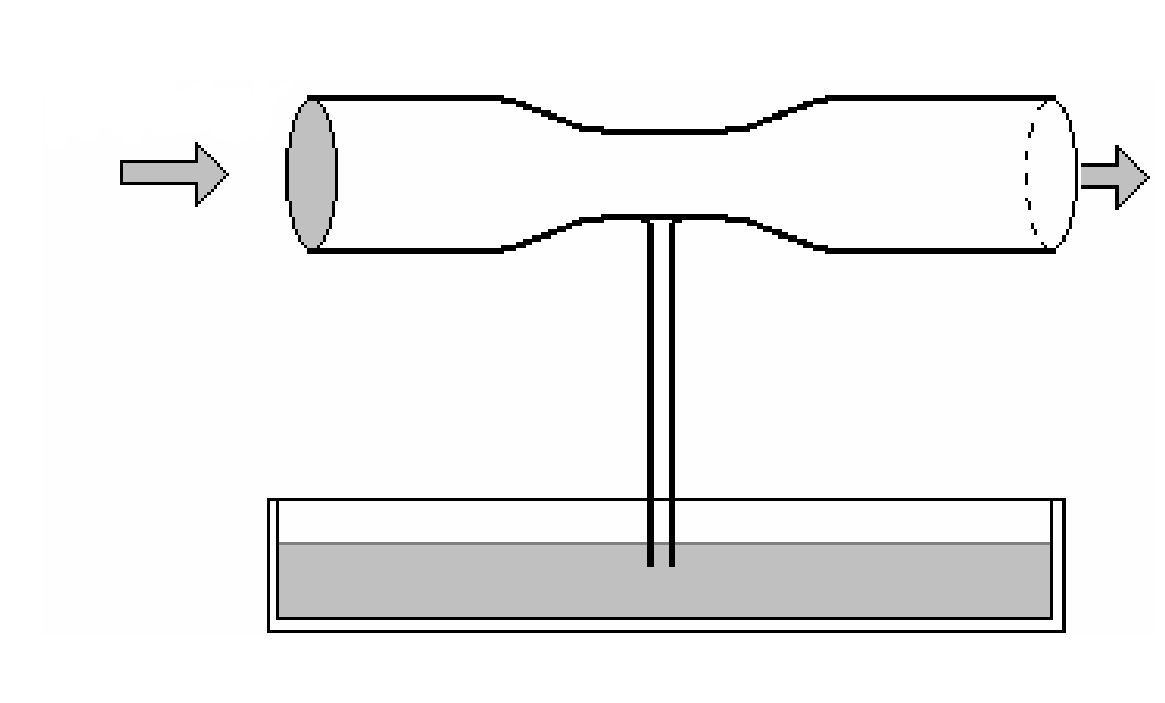
\includegraphics[width = 0.5\textwidth]{Rohr.jpg}
    \caption{Verengtes Rohr}
    \label{fig:Verengtes_Rohr}
  \end{figure}

  \begin{exercise}{Navier-Stokes}{10}
    Ein zylinderförmiger Stab mit Radius $R_1$ bewegt sich mit der Geschwindigkeit $u$
    parallel zu seiner Achse in einem zu ihm koaxialen zylinderförmigen Rohr mit Radius
    $R_2$. Der Raum zwischen dem Stab und dem Rohr ist mit einer inkompressiblen
    Flüssigkeit gefüllt. Die Strömung ist stationär.\\
    Wählen Sie an das Problem angepasste Zylinderkoordinaten $(r, \theta, z)$. Sie
    können davon ausgehen, dass die Geschwindigkeit $\vec{v}$ der Flüssigkeit nur von
    dem radialen Abstand von der Symmetrieachse abhängt und immer in $z$-Richtung zeigt
    (siehe Abbildung \ref{fig:Skizze_Koaxial}).

    \begin{enumerate}
      \item Welche Gleichung für $v_z$ erhalten Sie ausgehend von der Navier-Stokes-Gleichung?
      \item Welche Randbedingungen gelten? D.h. geben Sie $v_z(r = R_1)$ und $v_z(r = R_2)$ an.
      \item Lösen Sie die Navier-Stokes-Gleichung für diesen Fall. D.h. berechnen Sie $v_z(r)$.
    \end{enumerate}

    \begin{figure}[h]
      \centering
      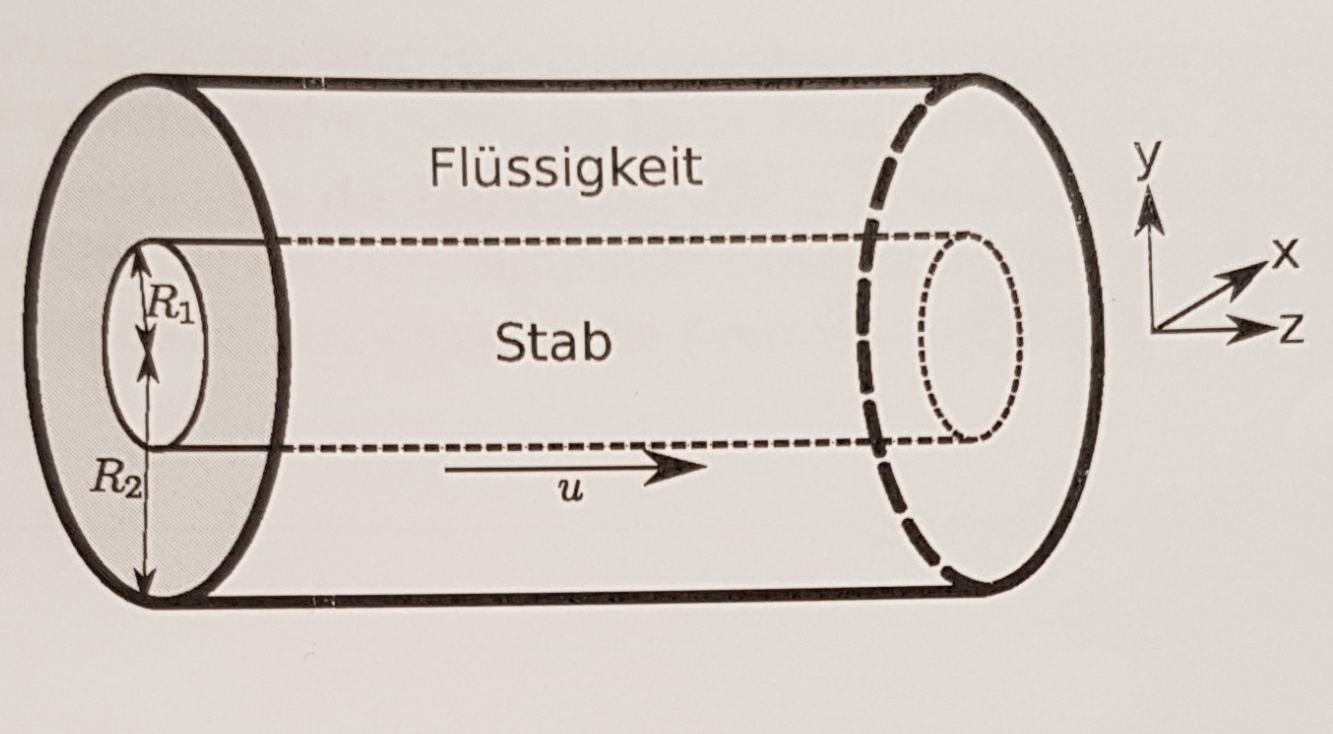
\includegraphics[width=0.7\textwidth]{Skizze_Navier_Stokes.jpg}
      \caption{Navier-Stokes}
      \label{fig:Skizze_Koaxial}
    \end{figure}

  \end{exercise}

\FloatBarrier
\newpage

\begin{exercise}{Zusatzaufgabe}{+10}
  \begin{enumerate}
    \item [a)] Bestimmen Sie das elektrische Feld eines unendlich langen geladenen Drahtes
               mit der Linienladungsdichte $\lambda$.
    \item [b)] Bestimmen Sie das magnetische Feld eines unendlich langen
               stromdurchflossenen Drahtes
               mit dem Radius $r_{0}$ und dem Strom I. Betrachten Sie dabei auch das Feld
               innerhalb des Leiters.
    \item [c)] Bestimmen Sie das magnetische Feld einer stromdurchflossenen
               Toroidspule mit innerem
               Radius $r_{1}$ und äu\ss erem Radius $r_{2}$. Die Spule hat N
               Windungen und wird vom Strom I durchflossen.
               Betrachten Sie dabei
               alle Bereiche (r<$r_{1}$,$r_{1}\leq r \leq r_{2}$,r>$r_{2}$).
  \end{enumerate}
\end{exercise}
\newpage

\begin{figure}[h]
  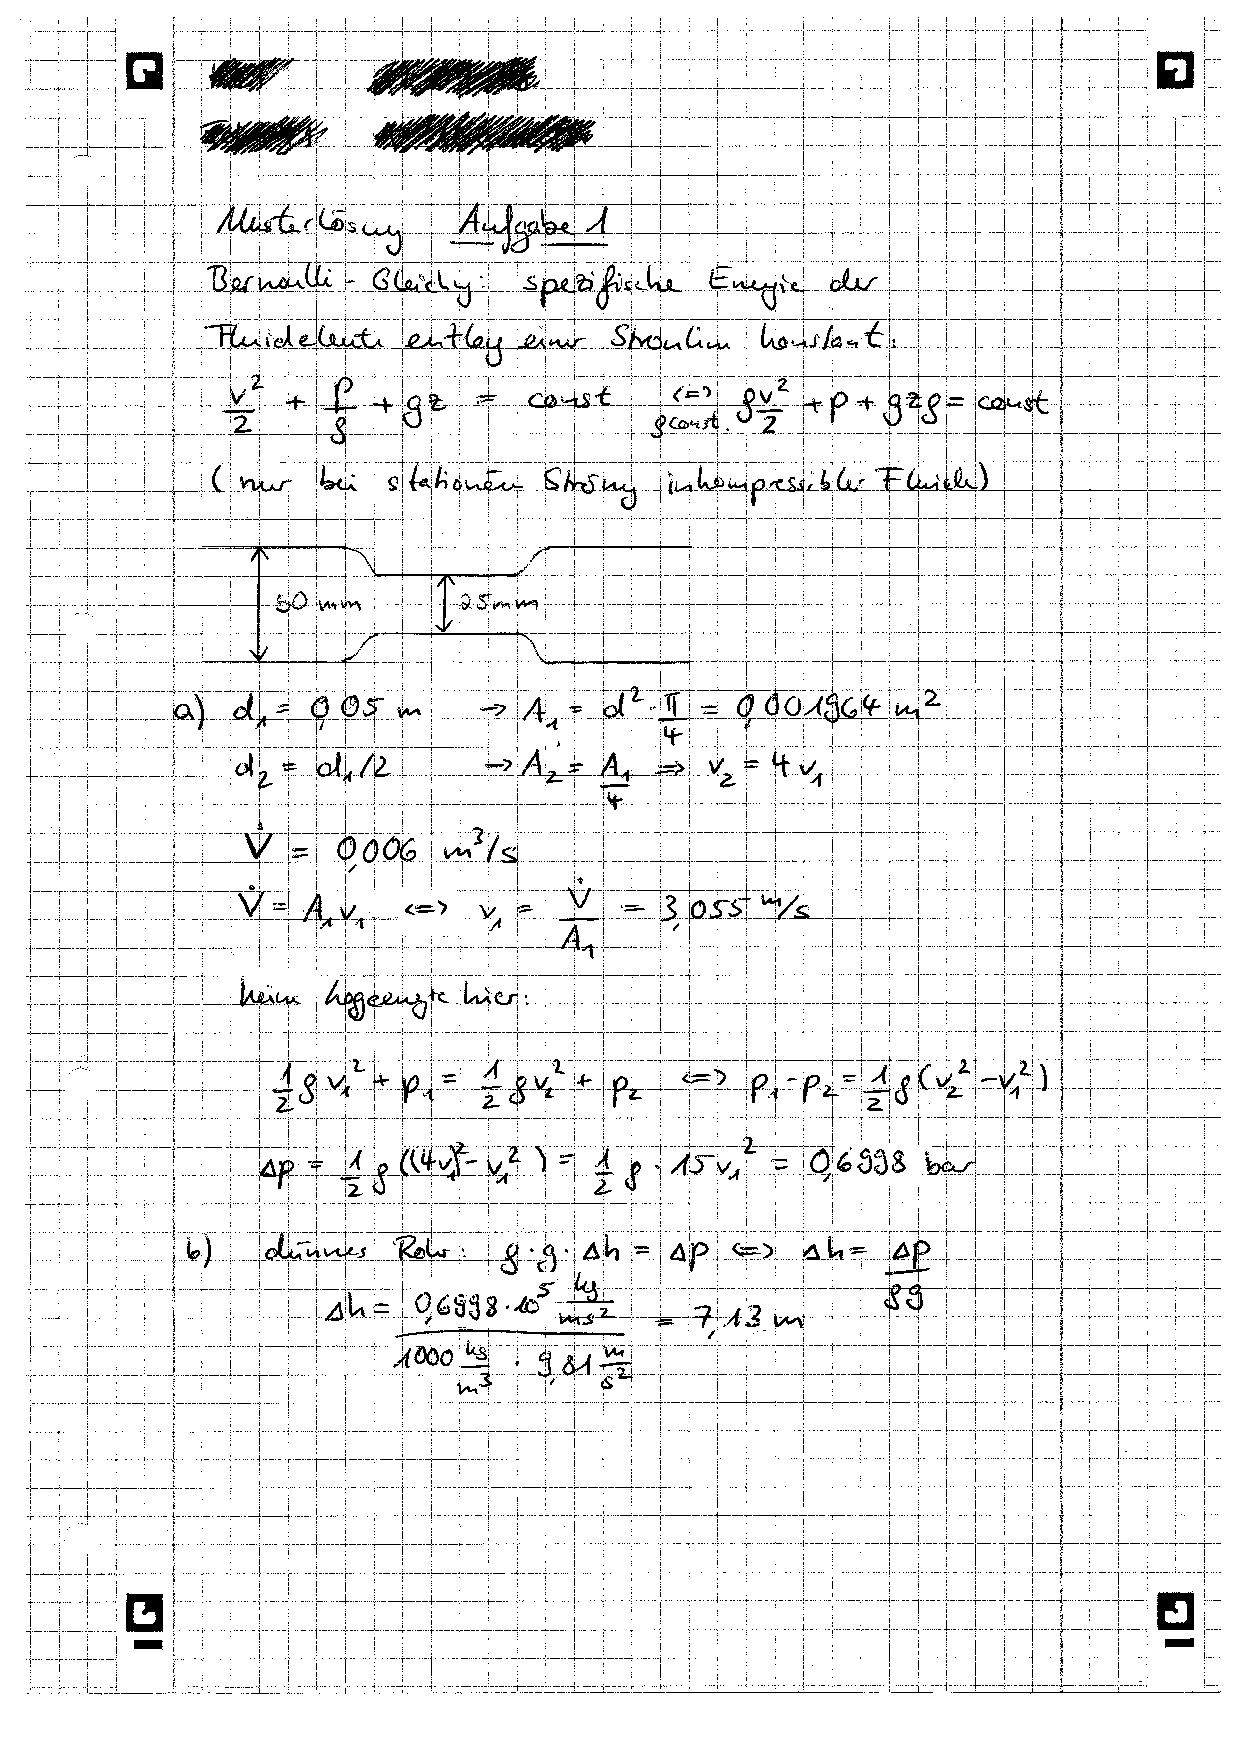
\includegraphics[width = \textwidth]{LoesungRohr.pdf}
\end{figure}

%%%%% MUSTERLÖSUNG %%%%%

\textbf{Musterlösung: Navier-Stokes}

\begin{itemize}
  \item[a.)]
    \begin{align*}
      v_x =& v_y = 0\\
      v_z =& v(r)\\
      \Rightarrow \Delta V =& \frac{1}{r}\frac{\text{d}}{\text{d}r}
      \left(r\frac{\text{d}v}{\text{d}r}\right) = 0
    \end{align*}
  \item[b.)]
    \begin{align*}
      v(r = R_1) =& u\\
      v(r = R_2) =& 0
    \end{align*}
  \item[c.)]
    \begin{align*}
      \frac{\text{d}}{\text{d}r}
      \left(r\frac{\text{d}v}{\text{d}r}\right) = 0\\
      \frac{\text{d}v}{\text{d}r} = \frac{c_1}{r}\\
      v(r) = c_1\cdot \ln{r} + c_2\\
      \text{Jetzt in die Randedingungen einsetzen:}\\
      \\
      u = v(R_1) =& c_1 \cdot \ln{R_1} + c_2\\
      0 = v(R_2) =& c_1 \cdot \ln{R_2} + c_2\\
      \Rightarrow c_1 = \frac{u}{\ln{\frac{R_1}{R_2}}} &
      c_2 = -\frac{u\ln{R_2}}{\ln{\frac{R_1}{R_2}}}\\
      \text{Ergebnis:}\\
      v(r) =& u\cdot\frac{\ln{\frac{r}{R_2}}}{\ln{\frac{R_1}{R_2}}}
    \end{align*}
\end{itemize}

\begin{figure}
  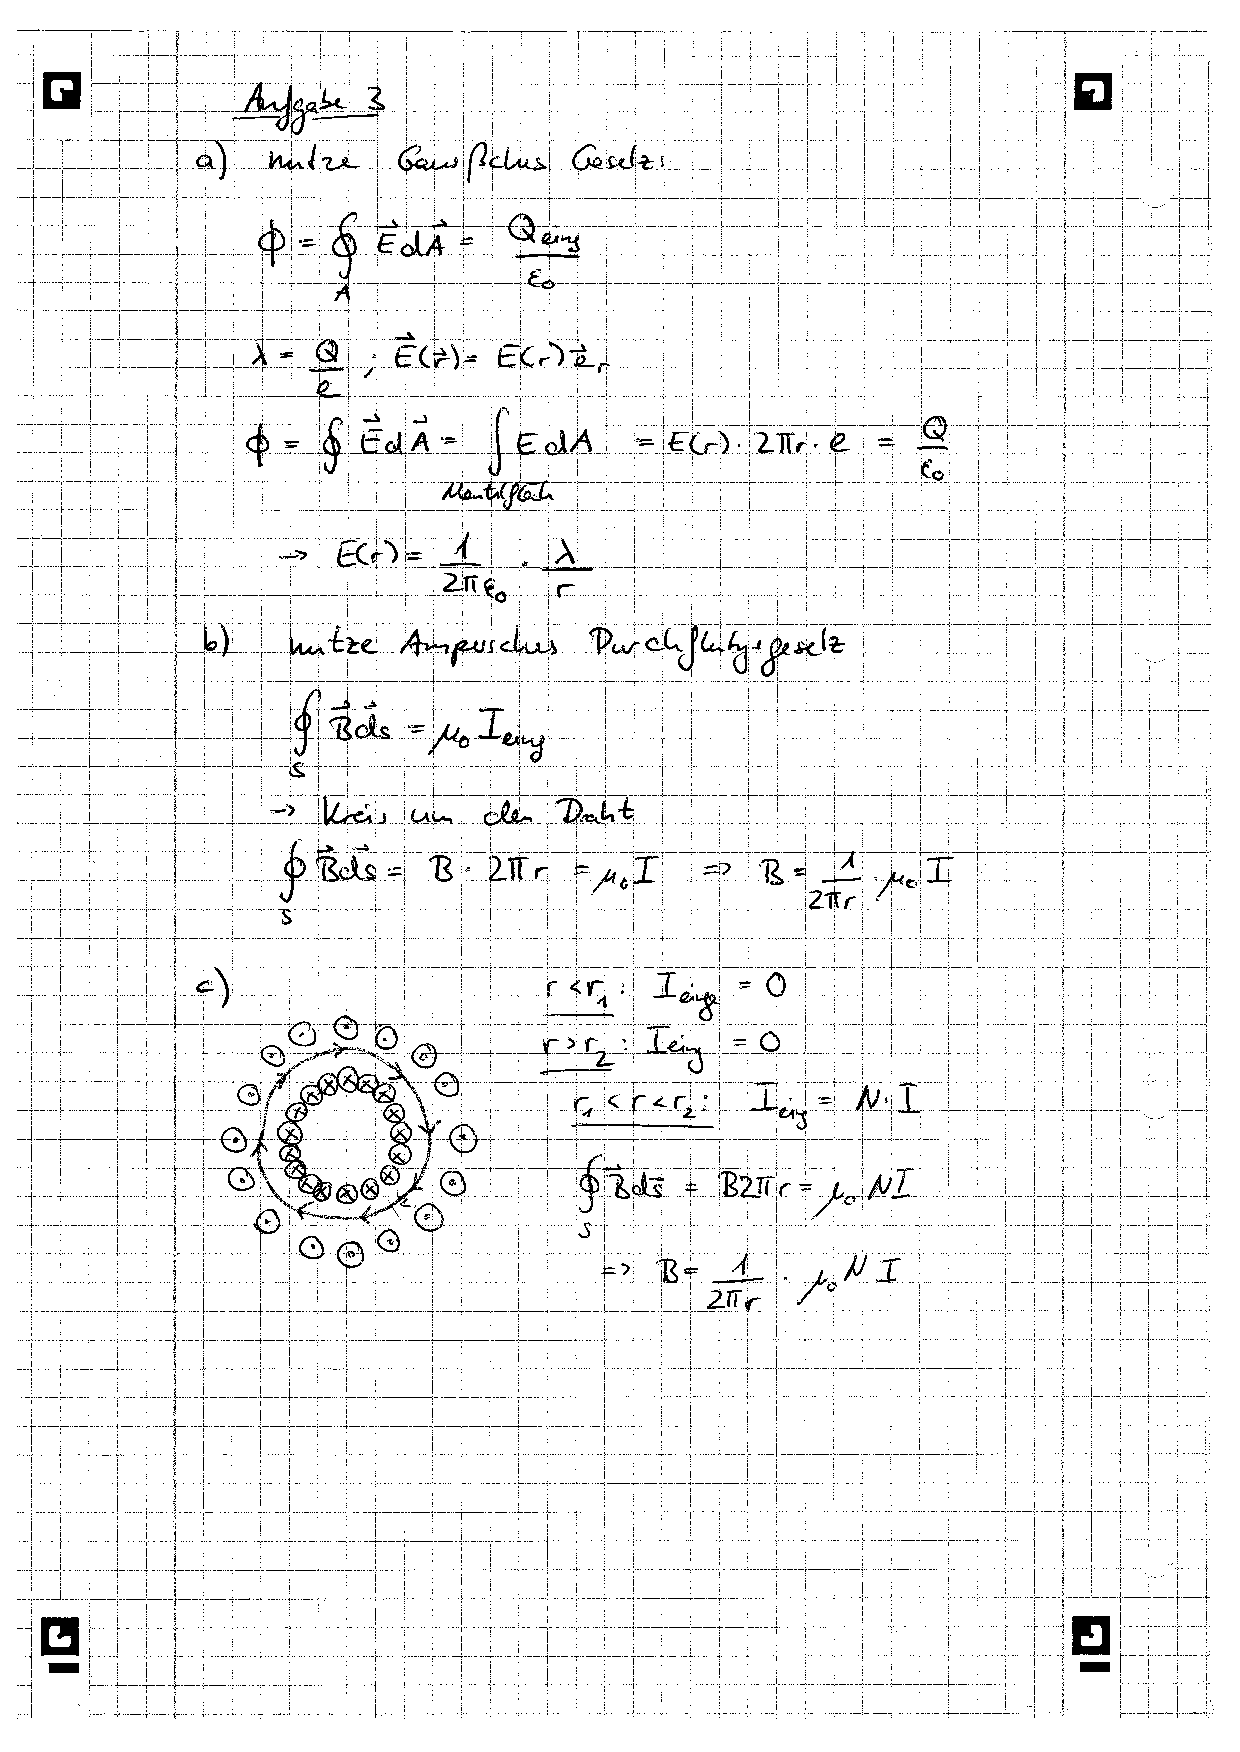
\includegraphics[width = \textwidth]{LoesungZusatz.pdf}
\end{figure}

\end{document}
